%% Copernicus Publications Manuscript Preparation Template for LaTeX Submissions
%% ---------------------------------
%% This template should be used for copernicus.cls
%% The class file and some style files are bundled in the Copernicus Latex Package which can be downloaded from the different journal webpages.
%% For further assistance please contact the Copernicus Publications at: publications@copernicus.org
%% http://publications.copernicus.org


%% Please use the following documentclass and Journal Abbreviations for Discussion Papers and Final Revised Papers.

%% 2-Column Papers and Discussion Papers
\documentclass[gmd, manuscript]{copernicus}

%% Journal Abbreviations (Please use the same for Discussion Papers and Final Revised Papers)

% Archives Animal Breeding (aab)
% Atmospheric Chemistry and Physics (acp)
% Advances in Geosciences (adgeo)
% Advances in Statistical Climatology, Meteorology and Oceanography (ascmo)
% Annales Geophysicae (angeo)
% ASTRA Proceedings (ap)
% Atmospheric Measurement Techniques (amt)
% Advances in Radio Science (ars)
% Advances in Science and Research (asr)
% Biogeosciences (bg)
% Climate of the Past (cp)
% Drinking Water Engineering and Science (dwes)
% Earth System Dynamics (esd)
% Earth Surface Dynamics (esurf)
% Earth System Science Data (essd)
% Fossil Record (fr)
% Geographica Helvetica (gh)
% Geoscientific Instrumentation, Methods and Data Systems (gi)
% Geoscientific Model Development (gmd)
% Geothermal Energy Science (gtes)
% Hydrology and Earth System Sciences (hess)
% History of Geo- and Space Sciences (hgss)
% Journal of Sensors and Sensor Systems (jsss)
% Mechanical Sciences (ms)
% Natural Hazards and Earth System Sciences (nhess)
% Nonlinear Processes in Geophysics (npg)
% Ocean Science (os)
% Proceedings of the International Association of Hydrological Sciences (piahs)
% Primate Biology (pb)
% Scientific Drilling (sd)
% SOIL (soil)
% Solid Earth (se)
% The Cryosphere (tc)
% Web Ecology (we)
% Wind Energy Science (wes)


%% \usepackage commands included in the copernicus.cls:
%\usepackage[german, english]{babel}
% \usepackage{tabularx}
%\usepackage{cancel}
%\usepackage{multirow}
%\usepackage{supertabular}
%\usepackage{algorithmic}
%\usepackage{algorithm}
%\usepackage{amsthm}
%\usepackage{float}
%\usepackage{subfig}
%\usepackage{rotating}
% \usepackage{graphicx}
\usepackage{hyperref}
\usepackage{tikz}
\usetikzlibrary{shapes.geometric, arrows, positioning, fit, calc}

% \DeclareGraphicsExtensions{.pdf, .png, .jpg, .eps}
\graphicspath{ {./figs/} }
%
% \usepackage{lineno}
% \linenumbers*[1]
%
% \begin{linenomath*}
% \begin{equation}
% \end{equation}
% \end{linenomath*}

% remove these lines before submission. I just don't like the really wide page that the default template uses
% start: remove
\addtolength{\evensidemargin}{1in}
\addtolength{\oddsidemargin}{1in}
\addtolength{\topmargin}{0.5in}
\addtolength{\textheight}{-1in}
\addtolength{\textwidth}{-2in}
% end: remove

\begin{document}

\title{The Variable Infiltration Capacity (VIC) Model, Version 5.0 - Improvements and New Applications}

% \Author[affil]{given_name}{surname}
\Author[1,2]{Joseph J.}{Hamman}
\Author[1]{Bart}{Nijssen}
\Author[3]{Theodore}{Bohn}
\Author[1]{Diana}{Gergel}
\Author[1]{Yixin}{Mao}

\affil[1]{Department of Civil \& Environmental Engineering, University of Washington, Seattle, WA, USA.}
\affil[2]{Now at: Hydrometeorological Applications Program, Research Applications Laboratory, National Center for Atmospheric Research, Boulder, Colorado, USA}
\affil[3]{School of Earth and Space Exploration, Arizona State University, Tempe, AZ, USA.}

%% The [] brackets identify the author with the corresponding affiliation. 1, 2, 3, etc. should be inserted.


\runningtitle{VIC version 5.1 - IMPROVEMENTS AND NEW APPLICATIONS}

\runningauthor{HAMMAN ET AL.}

\correspondence{Bart Nijssen (nijssen@uw.edu)}


\received{}
\pubdiscuss{} %% only important for two-stage journals
\revised{}
\accepted{}
\published{}

%% These dates will be inserted by Copernicus Publications during the typesetting process.

\firstpage{1}

\maketitle

\begin{abstract}
  The Variable Infiltration Capacity (VIC) model is a macro-scale semi-distributed hydrologic model. VIC development began in the early 1990s and the model has since been used extensively for basin- to global-scale applications that include hydrologic data set construction, trend analysis of hydrologic fluxes and states, data evaluation and assimilation, forecasting, coupled climate modeling, and climate change impact analysis. Ongoing operational applications of the VIC model include the University of Washington's drought monitor and forecast systems, and NASA's land data assimilation systems. This paper documents the development of VIC version 5 (VIC-5), which includes a major reconfiguration of the legacy VIC source code to support a wider range of modern hydrologic modeling applications. The VIC source code has been moved to a public GitHub repository to encourage participation by the broader user and developer communities. The reconfiguration has separated the core physics of the model from the driver source code, where the latter is responsible for memory allocation, pre- and post-processing and input/output (I/O). VIC-5 includes four drivers that use the same model physics core, but which allow for different methods for accessing this core to enable different model applications. Finally, VIC-5 is distributed with a robust test infrastructure, components of which routinely run during development using cloud-hosted continuous integration. The work described here provides an example to the model development community for extending the life of a legacy model that is being used extensively and represents a significant step forward for the VIC user community in terms of support for existing and new model applications, reproducibility, and scientific robustness.
\end{abstract}

\introduction
  The Variable Infiltration Capacity (VIC) model \citep{Liang_1994} is a macro-scale, semi-distributed hydrologic model (MHM) **a little confusing why this is abbreviated as MHM** which has been applied in a broad set of use cases. The model has been used for numerous water and energy balance studies in the U.S. \citep{Abdulla_1997,Nijssen_1997}, the arctic \citep{Adam_2008,Su_2005,Tan_2011,Hamman_2016a} and globally \citep{Nijssen_2001a,Nijssen_2001b,Nijssen_2001c,Sheffield_2009}. One result of these studies has been refinement of the model to better represent key hydrological processes \citep{Andreadis_2009,Cherkauer_2003,Liang_1996,Liang_1999}. Ongoing realtime applications of the VIC model include the University of Washington’s Drought Monitor and forecast systems (\url{http://hydro.washington.edu/forecast/monitor/drought/index.shtml}), and NASA’s land data assimilation systems (\url{http://ldas.gsfc.nasa.gov/nldas/}). Table \ref{table:vic_applications} provides additional examples of the use of VIC for hydrological, water resources, and water and energy budget applications.

  Although the motivation for the development of VIC, as documented in the original VIC publication \citep{Liang_1994}, was as a land surface scheme for coupled land-atmosphere models, the model has been applied predominantly in uncoupled modeling studies in which there is no feedback from the land surface to the atmosphere. These uncoupled MHMs have continued to exist alongside the fully coupled land surface schemes and have developed a large user community for a number of reasons: a) their focus on the representation of hydrological processes often resulted in simulations that were more hydrologically credible than the land surface schemes typically used in coupled land-atmosphere models (as shown, for instance, in the Project for Intercomparison of Land Surface Parameterizations (PILPS) \citep{Bowling_2003,wood_1998}); b) their ability to simulate variables that are directly relevant for water resources management, such as streamflow, makes them useful for planning and impact studies; and c) their lower demand for computational resources (compared with coupled models) allows research groups that do not have access to supercomputers to perform large-scale simulations. Most of these uncoupled MHMs can, for most applications, be run on single processors or small computer clusters.

  Because VIC was operated as a stand-alone land-surface scheme, there were no requirements for the model code to communicate with other model components in a coupled environment. In other words, there was no requirement for the model to \textit{"play well with others"}. {VIC applications within multi-model frameworks \citep[e.g. NASA LIS, ][]{Kumar_2006} have  required significant custom reconfiguration of the model interface. Instead, the model run-time environment focused on simplicity with the goal that VIC could run without the need for specific machine architectures, compilers or third-party libraries.} **I don't quite understand these two sentences** Model development prior to version 5 was directed primarily by the needs of specific model experiments and relatively little attention was paid to improvements of the model infrastructure, which had remained essentially unchanged since the early 1990s, including input/output (I/O) formats. As a consequence, model implementation typically required extensive reformatting and processing of model input and output files. Model changes were generally tested in ad-hoc fashion. While VIC model source code was versioned and publicly available since the early 1990s, model development was not always transparent. The source code repository of record resided on a private machine at the University of Washington.

  Although the ability to run MHMs such as VIC in uncoupled mode has been one of their strengths, earth system science has reached a point where the inability of some MHMs to be used in both coupled and uncoupled mode is a serious shortcoming. While some efforts have been made to couple VIC to both atmospheric and fully-coupled earth system models \citep[e.g.][]{Zhu_2009,Hamman_2016a}, these methods have been ad-hoc and required significant rewriting of the model infrastructure. In effect, this resulted in a version of the model code that was coupled, but which would rapidly become out-of-date relative to the uncoupled VIC version which was the main path for model enhancement and improvement.

  Interest in and advocacy for the use of established software development methods has grown in hydrology and the earth sciences to promote reproducibility of model and analysis results \citep[e.g.][]{Ceola_2015,Fienen_2016,Gil_2016,Hutton_2016}. Opinions differ with respect to the best workflows to promote reproducibility. For example, an active discussion ensued in response to the paper by \citet{Hutton_2016}, not so much about the need for improved workflows, but about implementation details and the required level of rigor \citep{Anel_2017,Melsen_2017,Hut_2017,Hutton_2017a,Hutton_2017b}. This debate takes place against a general discussion of the need for open source computer programs in science to increase scientific transparency in the model development and application process \citep{Ince_2012}. Improved model source code maintenance, standardized testing, and transparency forms only part of this drive towards greater reproducibility. Other elements include model and workflow documentation, versioning of data sets, and inclusion and standardization of metadata. **I'm a little confused about the point this paragraph is trying to make - what's the two sides of the debate? What are the takeaways?**

  This paper documents the development of VIC version 5, hereafter referred to as VIC-5, a new major release of the VIC model. The motivation for the development of VIC-5 is to extend VIC's useful life by adding the necessary infrastructure to allow the model to operate in a number of coupled and uncoupled modes, while relying on the same underlying physics implementations, and to ensure that upgrades to the physics routines are automatically available to all model configurations. In this paper we describe the software, infrastructure, and associated improvements in VIC-5 and provide baseline model diagnostics in terms of computational performance. The initial VIC-5 release does not add new or improved physical representations compared to the last release of the VIC-4 development track (version 4.2.d). Instead, the development of VIC-5 focused on reconfiguring the legacy VIC source code to support a wider range of modeling applications, to better integrate VIC with other applications, and to enhance reproducibility and source code maintenance.

  This paper is organized as follows. Sect.~\ref{sec:vic_infrastructure} briefly outlines the VIC legacy infrastructure in the model versions before VIC-5, details our design objectives, and discusses the major infrastructure changes implemented to meet those objectives. Sect.~\ref{sec:vic-5_simulations} includes results from test simulations with the new model code. Sect.~\ref{sec:vic_community} discusses our efforts to create and maintain a VIC community and to share the code. Concluding remarks are provided in Sect.~\ref{sec:conclusions}.

\section{VIC Infrastructure}
  \label{sec:vic_infrastructure}
  \subsection{Legacy Implementation}
    \label{sec:vic_legacy}

  Although VIC was originally developed to function as a land surface component in ESMs **ESM not defined?** \citep{Liang_1994}, its use has been overwhelmingly centered on stand-alone hydrologic modeling applications. As a result, many of the infrastructure features common in modern ESM component models, such as coupling with atmospheric components, parallel processing, and  standardized I/O, were never incorporated into the VIC source code. While a few applications of VIC within ESMs have been completed \citep{Zhu_2009,Hamman_2016a}, the required changes to the model infrastructure were so sweeping that they were never included in future releases of VIC.

  While the lack of infrastructure development may have made coupling within ESMs prohibitively difficult, it may have also contributed to the model's wide uptake throughout the hydrologic modeling community. Previous versions of VIC were very portable (required no third-party libraries), easy to run in single point mode for testing or comparison with point observations, and trivial to parallelize across many machines. It was this simple infrastructure, combined with the inclusion of built-in convenience tools such as the MT-CLIM \citep{Thornton_1999,Bohn_2013} meteorologic variable disaggregator and the availability of forcing and parameter datasets, that resulted in VIC's wide adoption in they hydrologic modeling community.

  \subsection{Updates in VIC-5}
    \label{sec:vic-5}
    The VIC-5 release includes a complete refactor of the model source code. The design goals of the refactor included: 1) enable the use of multiple model drivers to support a range of modeling applications, 2) support parallel processing to enable large domain simulations, 3) facilitate the use of modern I/O formats such as NetCDF, 4) develop a comprehensive test suite to guide future model use and development, and 5) provide the user community with improved model documentation.

    A pratical motivating factor in the development of VIC-5 was to enable coupling of VIC within the Regional Arctic System Model \citep[RASM;][]{Hamman_2016a}, a regional implementation of the Community Earth System Model \citep[CESM;][]{Hurrell_2013}, while maintaining usability as a stand-alone model. In RASM, VIC-5 is directly coupled to CESM's flux coupler \citep[CPL7;][]{Craig_2012} via the Model Coupling Toolkit interface \citep[MCT;][]{Larson_2005}. The new interface in VIC-5 allows VIC to be tightly-coupled to atmospheric and streamflow routing model components (WRF and RVIC in the case of RASM), while maintaining legacy and stand-alone model infrastructure. The successful coupling of VIC-5 within RASM is a key demonstration of the benefits of the source code refactor. In the future, VIC may also be readily coupled to other third-party modeling systems, such as WRF-Hydro or NASA's LIS.

  \subsection{Drivers}
    \label{sec:drivers}
    The most significant change in the model reconfiguration was the separation of the physical core of the model from the driver, which is responsible for memory allocation, pre- and post-processing, and input and output (I/O). The VIC-5 source code structure is depicted in Fig.~\ref{fig:vic_config}. The initial VIC-5 release includes four drivers, each using the same physical model core:

  \begin{enumerate}
    \item  The \textit{Classic Driver} supports legacy VIC configurations and runs in the traditional time-before-space configuration (i.e., simulation is done for the entire time period of simulation at a spatial location before moving to the next location). It uses the ASCII and flat-binary file formats for I/O.

    \item The \textit{Image Driver} includes a stand-alone space-before-time configuration (i.e., one timestep of simulation is done for the entire spatial domain before moving to the next timestep), NetCDF I/O \citep{Rew_1990}, and uses MPI and OpenMP for parallel processing \citep{Gropp_1996}. This configuration facilitates the direct coupling of streamflow routing, reservoir, and irrigation processes within VIC which requires spatial knowledge of hydrologic conditions.

    \item The \textit{CESM Driver} couples VIC to Community Earth System Model's \citep[CESM;][]{Hurrell_2013} flux coupler \citep[CPL7;][]{Craig_2012} and a prognostic atmosphere. The initial application of the \textit{CESM Driver} is within the Regional Arctic System Model (RASM) \citep{Hamman_2016a}, a regional implementation of CESM. Future applications of the \textit{CESM Driver} may be readily applied within the global version of CESM. Furthermore, the CESM driver may serve as a template for other coupled model applications as it provides the infrastructure necessary to couple VIC, which is written in C, to Fortran libraries. The \textit{CESM Driver} shares much of its foundational infrastructure with the \textit{Image Driver}. In particular, they share common source code for their parallelization and I/O layers. See Fig.~\ref{fig:vic_config} for illustration of the shared infrastructure between the Image Driver and the CESM Driver.

    \item The \textit{Python Driver} provides Python bindings to the functions and datatypes of VIC’s physical core. These functions are made available as Python functions using the C Foreign Function Interface for Python (CFFI; \url{http://cffi.readthedocs.io/}). Although the \textit{Python Driver} is currently only used for testing, this driver is uniquely suited for future interactive classroom, data assimilation, or large ensemble applications.

  \end{enumerate}

  **Maybe add a separate section to describe the extension structure, with emphasis of the convenience for adding new extension features under the current framework**
  We have also introduced a model extensions framework to facilitate the coupling of sub-model components, such as streamflow routing, reservoirs, irrigation, glaciers and ice sheets, and dynamic vegetation and crops. The motivating factor for developing this framework was to allow for the optional coupling of existing sub-models that are beyond the scope of core VIC applications or that are not feasible to add for all drivers. These extensions are designed to be enabled via compile time options. At the time of writing, only the streamflow routing extension, which couples the RVIC streamflow routing model \citep{Hamman_2017a} to the \textit{Image Driver}, is complete.

  \subsection{Parallel Computing}
    \label{sec:parallel}
    The VIC model does not include horizontal transport between grid cells. In the past, this feature has allowed users to manually parallelize their VIC applications by running VIC simulations on completely separate cores or computers for different grid cells, if need be. In the image and CESM drivers in VIC-5, we have added formal parallel processing support utilizing the Message Passing Interface (MPI) standard \citep{Gropp_1996} and shared memory threading via OpenMP \citep{Dagum_1998}. Leveraging the independence of VIC grid points in terms of neighbor communication (i.e. no horizontal transport between grid cells), the parallelization strategy that we have adopted only uses MPI utilities to facilitate I/O operations, while the core physics for grid cells is simply run on multiple cores/machines without the need of message passing. Shared memory between MPI tasks is limited to model settings. OpenMP threading may be used for concurrent simulation of multiple grid cells within a single MPI task. The parallel scaling performance of the VIC-5 image driver is discussed in detail in Sect. \ref{sec:vic-5_simulations}.

  \subsection{Input and Output}
    \label{sec:io}
    The Image and CESM drivers use Unidata's Network Commmon Data Format (NetCDF) **"NetCDF" has appeared above; move the full name to the first time of appearance** library for all I/O related to input parameters, meteorological forcings, and model output. NetCDF is a software library that reads and writes array-oriented scientific data with metadata. It has been widely adopted among the geo-scientific modeling community and provides a convenient self-describing machine-independent data format. Interfaces to the NetCDF library are available in many scripting languages including Python, R, Matlab, and Julia. Output files from the Image and CESM drivers are formatted such that they meet the NetCDF Climate and Forecast (CF) metadata conventions version 1.6 \citep{Eaton_2003}.

    The classic driver continues to support the legacy ASCII and raw binary input and output file formats. We have also added additional metadata to the ASCII file formats but they have basically remained the same since VIC-4.

    VIC-5 also has eliminated all hard-coded model parameters from the body of the source code **maybe give a few examples of parameters for easier understanding?**. Users may now specify an optional ``parameters'' configuration file to override default model constants that were previously hard-coded values. Following \citet{Mendoza_2015} call for hydrologic models to expose constant parameters, this change greatly improves the transparency, flexibility, and accessibility of the model.

  \subsection{Testing}
    \label{sec:testing}
    VIC-5 introduces a much more comprehensive test suite, now distributed with the model source code. The test suite is made up of six components:

    \begin{enumerate}
      \item \textit{Unit}: Unit tests are tests that check function-level source code behavior. Using the \textit{Python Driver}, many of the individual functions in VIC are tested by using the ``Py-Test'' unit test framework (\url{http://doc.pytest.org/}).

      \item \textit{System}: The system tests check the behavior of the individual drivers. Examples of these tests include checks for exact restarts using model generated state files, binary equivalence for simulations run with and without parallel processing, and comparisons between drivers.

      \item \textit{Science}: The science tests utilize the classic driver to run point simulations at a selection of observation locations (e.g. SNOTEL or AMERIFLUX). Results from these point simulations are quantitatively and qualitatively compared to observations and also to simulation results from previous VIC versions. Fig.~\ref{fig:vic_4v5} provides an example of aggregated output from the science tests suite.

      \item \textit{Examples}: A set of short example VIC configurations and inputs are provided to users for the Classic and Image drivers. The Examples tests simply check that the example data continue to run so that users can quickly and easily get started with the VIC model.

      \item \textit{Release}: The release tests are longer, full domain (e.g. North America, Global, etc.) simulations performed prior to each model release. These tests demonstrate the current model behavior and are compared to previous releases to demonstrate the changes in the model physics. These tests are archived for retrospective model comparison.

      \item \textit{Performance}: With the addition of parallel processing to the Image and CESM drivers, a set of tools for assessing the parallel performance were needed. The performance tests asses timing and memory statistics of the VIC model. Results from these tests are highlighted in Sect. \ref{sec:vic-5_simulations}.
    \end{enumerate}

    **Maybe move this overview of test suite up to before the detailed explanation of the 6 tests?**The VIC test suite was designed to serve two primary purposes: 1) automated diagnostics and benchmarking of model performance with similar coverage to what is provided in the ILAMB project \citep{Luo_2012}, and 2) automated build and unit tests to ensure reproducibility and facilitate consistency between model developers. The \textit{Unit}, \textit{System}, and \textit{Examples} tests are routinely run using the Travis CI continuous integration system (\url{https://travis-ci.org/UW-Hydro/VIC}) where the VIC test suite is tested against a series of compilers and computational architectures. As the VIC developer community continues to grow, this test suite will be an important tool in maintaining the function of the supported drivers.

  \section{VIC-5 Simulations}
    \label{sec:vic-5_simulations}
	**Maybe have three subsections in this section: 1) science tests; 2) release tests; 3) scaling tests.**
    The science and release tests described above were performed prior to releasing VIC-5. The scientific validation of the VIC-5 release included point comparisons of VIC simulations with 66 FluxNET [TED - provide citation] observations and 448 SNOTEL [citation?] observations. DIANA: please fill in this Section a bit more. We want to highlight why we use the datasets we do and where they are located.

	**Put the texts from here down under subsection 3 (scaling tests)**
    In this paper, we demonstrate the parallel scaling performance of the \textit{Image Driver} using a series of model simulations on the 50-km near equal area RASM domain. This model domain is shown in Fig.~\ref{fig:vic_domain} and is detailed in Table \ref{table:tests}. Here we demonstrate the scaling performance of the parallelization scheme applied in VIC-5 where model throughput **explain what throughput is** is shown as a function of the size of the HPC **first use of "HPC" - show full name** resources used. Two RASM image driver model configurations were tested on two super-computers, \verb|Thunder| and \verb|Cheyenne|. Table \ref{table:hardware} provides details on the hardware specifications of each machine. The different model configurations represent two ends of the complexity spectrum available in the VIC model. Configuration A was run in water balance mode, where the energy balance is not explicitly closed, resulting in a less expensive model. Conversely, configuration B represents a much more complex model where the energy and water budgets are solved together using an interative solver. Both configurations are run over the same model domain with the same meteorological forcings, with the only differences being model configuration options. Because memory usage is modest in VIC (it is basically a 2d model **why is VIC a 2-D model? Also why does a 2-D model have modest memory usage?**), parallelization with MPI is mainly for computational speedup and to facilitate I/O, allowing for centralized reads and writes. In most cases, the scaling  is mostly a function of the computer's interconnect and disk speed.

    Fig.~\ref{fig:vic_scaling} demonstrates the scaling performance for the two model configurations. For the simpler model configuration (A), VIC has remarkably high throughput but parallelization beyond one node provides no further speedup. This behavior is indicative of a program that is I/O limited. For the more complex model configuration (B), VIC has significantly lower throughput, but is shown to scale out efficiently beyond 288 processors. In this case, the computation time inside of the physics code of VIC is much higher than the I/O portions of the model **show some actual data to support this, if possible**.

    We expect the scaling performance of the VIC image and CESM drivers to be further improved by the application of parallel I/O **I'm a little confused whether I/O is parallelized in VIC-5. This paragraph seems to indicate that the current version does not parallelize I/O, but the texts above (as well as when describing the CESM driver in section 2.3) seem to suggest that it does parallelize I/O.**. Collective parallel reading and writing of NetCDF files, made possible through the NetCDF-4 and HDF5 libraries, are expected to dramatically reduce the amount of data passed via MPI processes and, for computers with high-performance parallel disks, should allow the model to scale well beyond the limits shown in Fig.~\ref{fig:vic_scaling}. The development of this feature has been reserved for later versions in the VIC-5 development track.

  \section{The VIC Community and Open Source}
    \label{sec:vic_community}
	**What about giving one example of community contribution to VIC-5 (say, the routing extention, which is right now only briefly mentioned in section 2.3) in more detail to illustrate that the new VIC version allows for much more convenient collaboration and community contribution?**
    The VIC model continues to serve a broad user community. The VIC Users email list-serve (\url{vic_users@u.washington.edu}) has more than 420 active members, and the analytics from the VIC website and documentation indicates that there are upwards of one-thousand individual VIC users. Citations of the original VIC paper \citep{Liang_1994} continue to increase. Since the VIC source code has been available in a public GitHub repository, over 160 users have checked out ``Forks''. Additionally, we are aware of a multiple ongoing developing efforts by the VIC community to implement new features. The open source framework that we have implemented will facilitate mechanisms for the integration of model improvements from the greater VIC community into future VIC releases.

    Beginning in 2011, the VIC model has been licensed with the open source GNU General Public License version 2. The motivation behind making the model source code completely open-source was to encourage participation by the model user and development community-at-large, and to increase scientific transparency in the model development and application process \citep{Ince_2012}. The VIC source code now uses the Git version control system \citep{Torvalds_2010} and is publicly available on GitHub (\url{https://github.com/UW-Hydro/VIC}). While the majority of the VIC-5 development was done by researchers at the University of Washington, a number of features and bug fixes were made by unsolicited contributors.

\conclusions[Conclusions]
\label{sec:conclusions}
  **I think this conclusion section is better to be a summary of the advances of VIC-5. The details of science tests, extension, etc. can be moved up into previous sections.**
  **Shouldn't this paragraph be under section 3?**
  The inclusion of a comprehensive science testing framework within the VIC-5 repository, as introduced in Sect.~\ref{sec:testing}, facilitates continuous and repeatable validation of the model throughout the development process. Fig.~\ref{fig:vic_4v5} shows a summary figures from the VIC SNOTEL portion of science testing package. This figure demonstrates that VIC-4 and VIC-5 are producing basically identical (r2 > 0.99) results and the two model versions have similar performance statistics when compared to observations (x and y respectively). Fig.~\ref{fig:vic_fluxes} demonstrates an example comparison from the FLUXNET portion of the science testing package, showing a comparison between VIC and flux tower observations for a subset of the sites included in the dataset.

  **Shouldn't this paragraph be under section 2 when describing extension?**
  The updated model configuration facilitates the direct coupling of new and existing subcomponents to VIC. Work currently underway is using the extensions framework discussed in Sect.~\ref{sec:vic-5} to tightly couple additional extensions, namely reservoir operations and irrigation, with the image driver \citep{Hamman_2017a}. Future extension development is also expected to add glaciers, dynamic vegetation, and crop models to VIC. While some of these had been partially developed with VIC-4, the limitations imposed by the lack of infrastructure have preclude their wider application in the VIC community.

  With the open-source status of VIC and the release of VIC-5, we hope to see growing community activity in the maintenance and development of the model. The reconfiguration of the model source code and the addition of an extensions framework will support a range of model developments.

\section{Code Availability}
\label{appendix:code_avail}

  Appendix \ref{appendix:source_code} describes the locations and license information for the the VIC source code and documentation. The source code, input data, and VIC configurations used as demonstrations for this paper, are provided in this GitHub repository: \url{https://github.com/jhamman/VIC5_paper}.

\appendix
\section{VIC Model Source Code and Documentation}
\label{appendix:source_code}

**Make "Archive" have the same indent as "Code Repository" and "Versioned Documentation"**
{\bf Archive}

\begin{itemize}
	\item \textit{Name}: VIC.5.1.0
	\item \textit{Persistent identifier}: 10.5281/zenodo.267178
	\item \textit{License}: GNU General Public License, version 2 (GPL-2.0)
	\item \textit{Publisher}:  Zenodo
	\item \textit{Version published}: 5.1.0
	\item \textit{Date published}: February 1, 2017
\end{itemize}

{\bf Code Repository}

\begin{itemize}
	\item \textit{Name}: GitHub
	\item \textit{Identifier}: \url{https://github.com/UW-Hydro/VIC}
	\item \textit{License}: GNU General Public License, version 2 (GPL-2.0)
	\item \textit{Date published}: February 1, 2017
\end{itemize}

{\bf Versioned Documentation}

\begin{itemize}
	\item \textit{Name}: ReadTheDocs
	\item \textit{Identifier}: \url{http://vic.readthedocs.io/en/vic.5.1.0}
	\item \textit{License}: GNU General Public License, version 2 (GPL-2.0)
	\item \textit{Date published}: February 1, 2017
\end{itemize}

% \subsection{}                               %% Appendix A1, A2, etc.

\authorcontribution{J. Hamman, B. Nijssen, and T. Bohn performed the majority the source code reconfiguration. B. Nijssen provided overall oversight. J. Hamman designed the experiments with help from Y. Mao and D. Gergel to carry them out. J. Hamman and B. Nijssen prepared the manuscript with contributions from all co-authors.}

\begin{acknowledgements}
  This research was supported, in part, by United States Department of Energy (DOE) grants DE-FG02-07ER64460 and DE-SC0006856 to the University of Washington, and grant 1216037 of the National Science Foundation's Science, Engineering, and Education for Sustainability (SEES) Program. We thank Anthony Craig for his feedback during the design and implementation of the Image and CESM drivers. **Should we thank Wietse's group?**
\end{acknowledgements}


%% REFERENCES

%% The reference list is compiled as follows:

% \begin{thebibliography}{}
%
% \bibitem[AUTHOR(YEAR)]{LABEL}
% REFERENCE 1
%
% \bibitem[AUTHOR(YEAR)]{LABEL}
% REFERENCE 2
%
% \end{thebibliography}

%% Since the Copernicus LaTeX package includes the BibTeX style file copernicus.bst,
%% authors experienced with BibTeX only have to include the following two lines:
%%
\bibliographystyle{copernicus}
\bibliography{biblio}
%%
%% URLs and DOIs can be entered in your BibTeX file as:
%%
%% URL = {http://www.xyz.org/~jones/idx_g.htm}
%% DOI = {10.5194/xyz}


%% LITERATURE CITATIONS
%%
%% command                        & example result
%% \citet{jones90}|               & Jones et al. (1990)
%% \citep{jones90}|               & (Jones et al., 1990)
%% \citep{jones90,jones93}|       & (Jones et al., 1990, 1993)
%% \citep[p.~32]{jones90}|        & (Jones et al., 1990, p.~32)
%% \citep[e.g.,][]{jones90}|      & (e.g., Jones et al., 1990)
%% \citep[e.g.,][p.~32]{jones90}| & (e.g., Jones et al., 1990, p.~32)
%% \citeauthor{jones90}|          & Jones et al.
%% \citeyear{jones90}|            & 1990



%% FIGURES

%% ONE-COLUMN FIGURES

%%f
\clearpage
\tikzstyle{driver} = [rectangle, rounded corners, minimum width=2cm, minimum height=1cm,text centered, draw=black, fill=gray!60]
\tikzstyle{extension} = [rectangle, rounded corners, minimum width=2cm, minimum height=1cm,text centered, draw=black]
\tikzstyle{shared} = [rectangle, rounded corners, minimum width=4cm, minimum height=1cm,text centered, draw=black, fill=gray!30]

\begin{figure}[t]
\centering
\begin{tikzpicture}
    \node (classic) [driver] {Classic Driver};
    \node (image) [driver, right of=classic, xshift=1.5cm] {Image Driver};
    \node (cesm) [driver, right of=image, xshift=1.5cm] {CESM Driver};
    \node (python) [driver, right of=cesm, xshift=1.5cm] {Python Driver};

    \node (shared) [shared, fit=(image)(cesm),below=of image.south west, anchor=north west, inner sep=0, yshift=0.5cm] {Shared Image Driver};

    \node (ext1) [extension, below of=classic, yshift=-2cm] {Extensions};
    \node (ext2) [extension, below of=image, yshift=-2cm] {Extensions};
    \node (ext3) [extension, below of=cesm, yshift=-2cm] {Extensions};
    \node (ext4) [extension, below of=python, yshift=-2cm] {Extensions};

    \node (shared) [shared, fit=(ext1)(ext4),below=of ext1.south west,anchor=north west, inner sep=0, yshift=0.5cm] {Shared Driver Utilities};
    \node (vic_run) [shared, fit=(ext1)(ext4),below=of shared.south west,anchor=north west, inner sep=0, yshift=0.5cm, fill=green!30] {VIC Physical Core};

    \draw[thick,dotted] ($(classic.north west)+(-0.5,0.15)$) rectangle ($(shared.south east)+(0.5,-0.15)$);


\end{tikzpicture}
\caption{The reconfigured VIC-5 source code structure. The ``Physical Core'' includes the scientific modules of VIC (e.g. routines that simulate the fluxes and states of the model) and is used by all drivers. The remainder of the VIC source code structure is considered driver-level code. Each driver uses components of the ``Shared Driver'' to minimize code duplication at the driver level. Likewise, the ``Shared Image Driver'' includes source code that is used by both the Image and CESM drivers (e.g. MPI and NetCDF utilities). Finally, the ``Extensions'' constitutes optional and driver specific sub-models.}
\label{fig:vic_config}
\end{figure}


\clearpage
\begin{figure}[t]
**I agree that it'd be better to show results from VIC-5 release test for this figure**
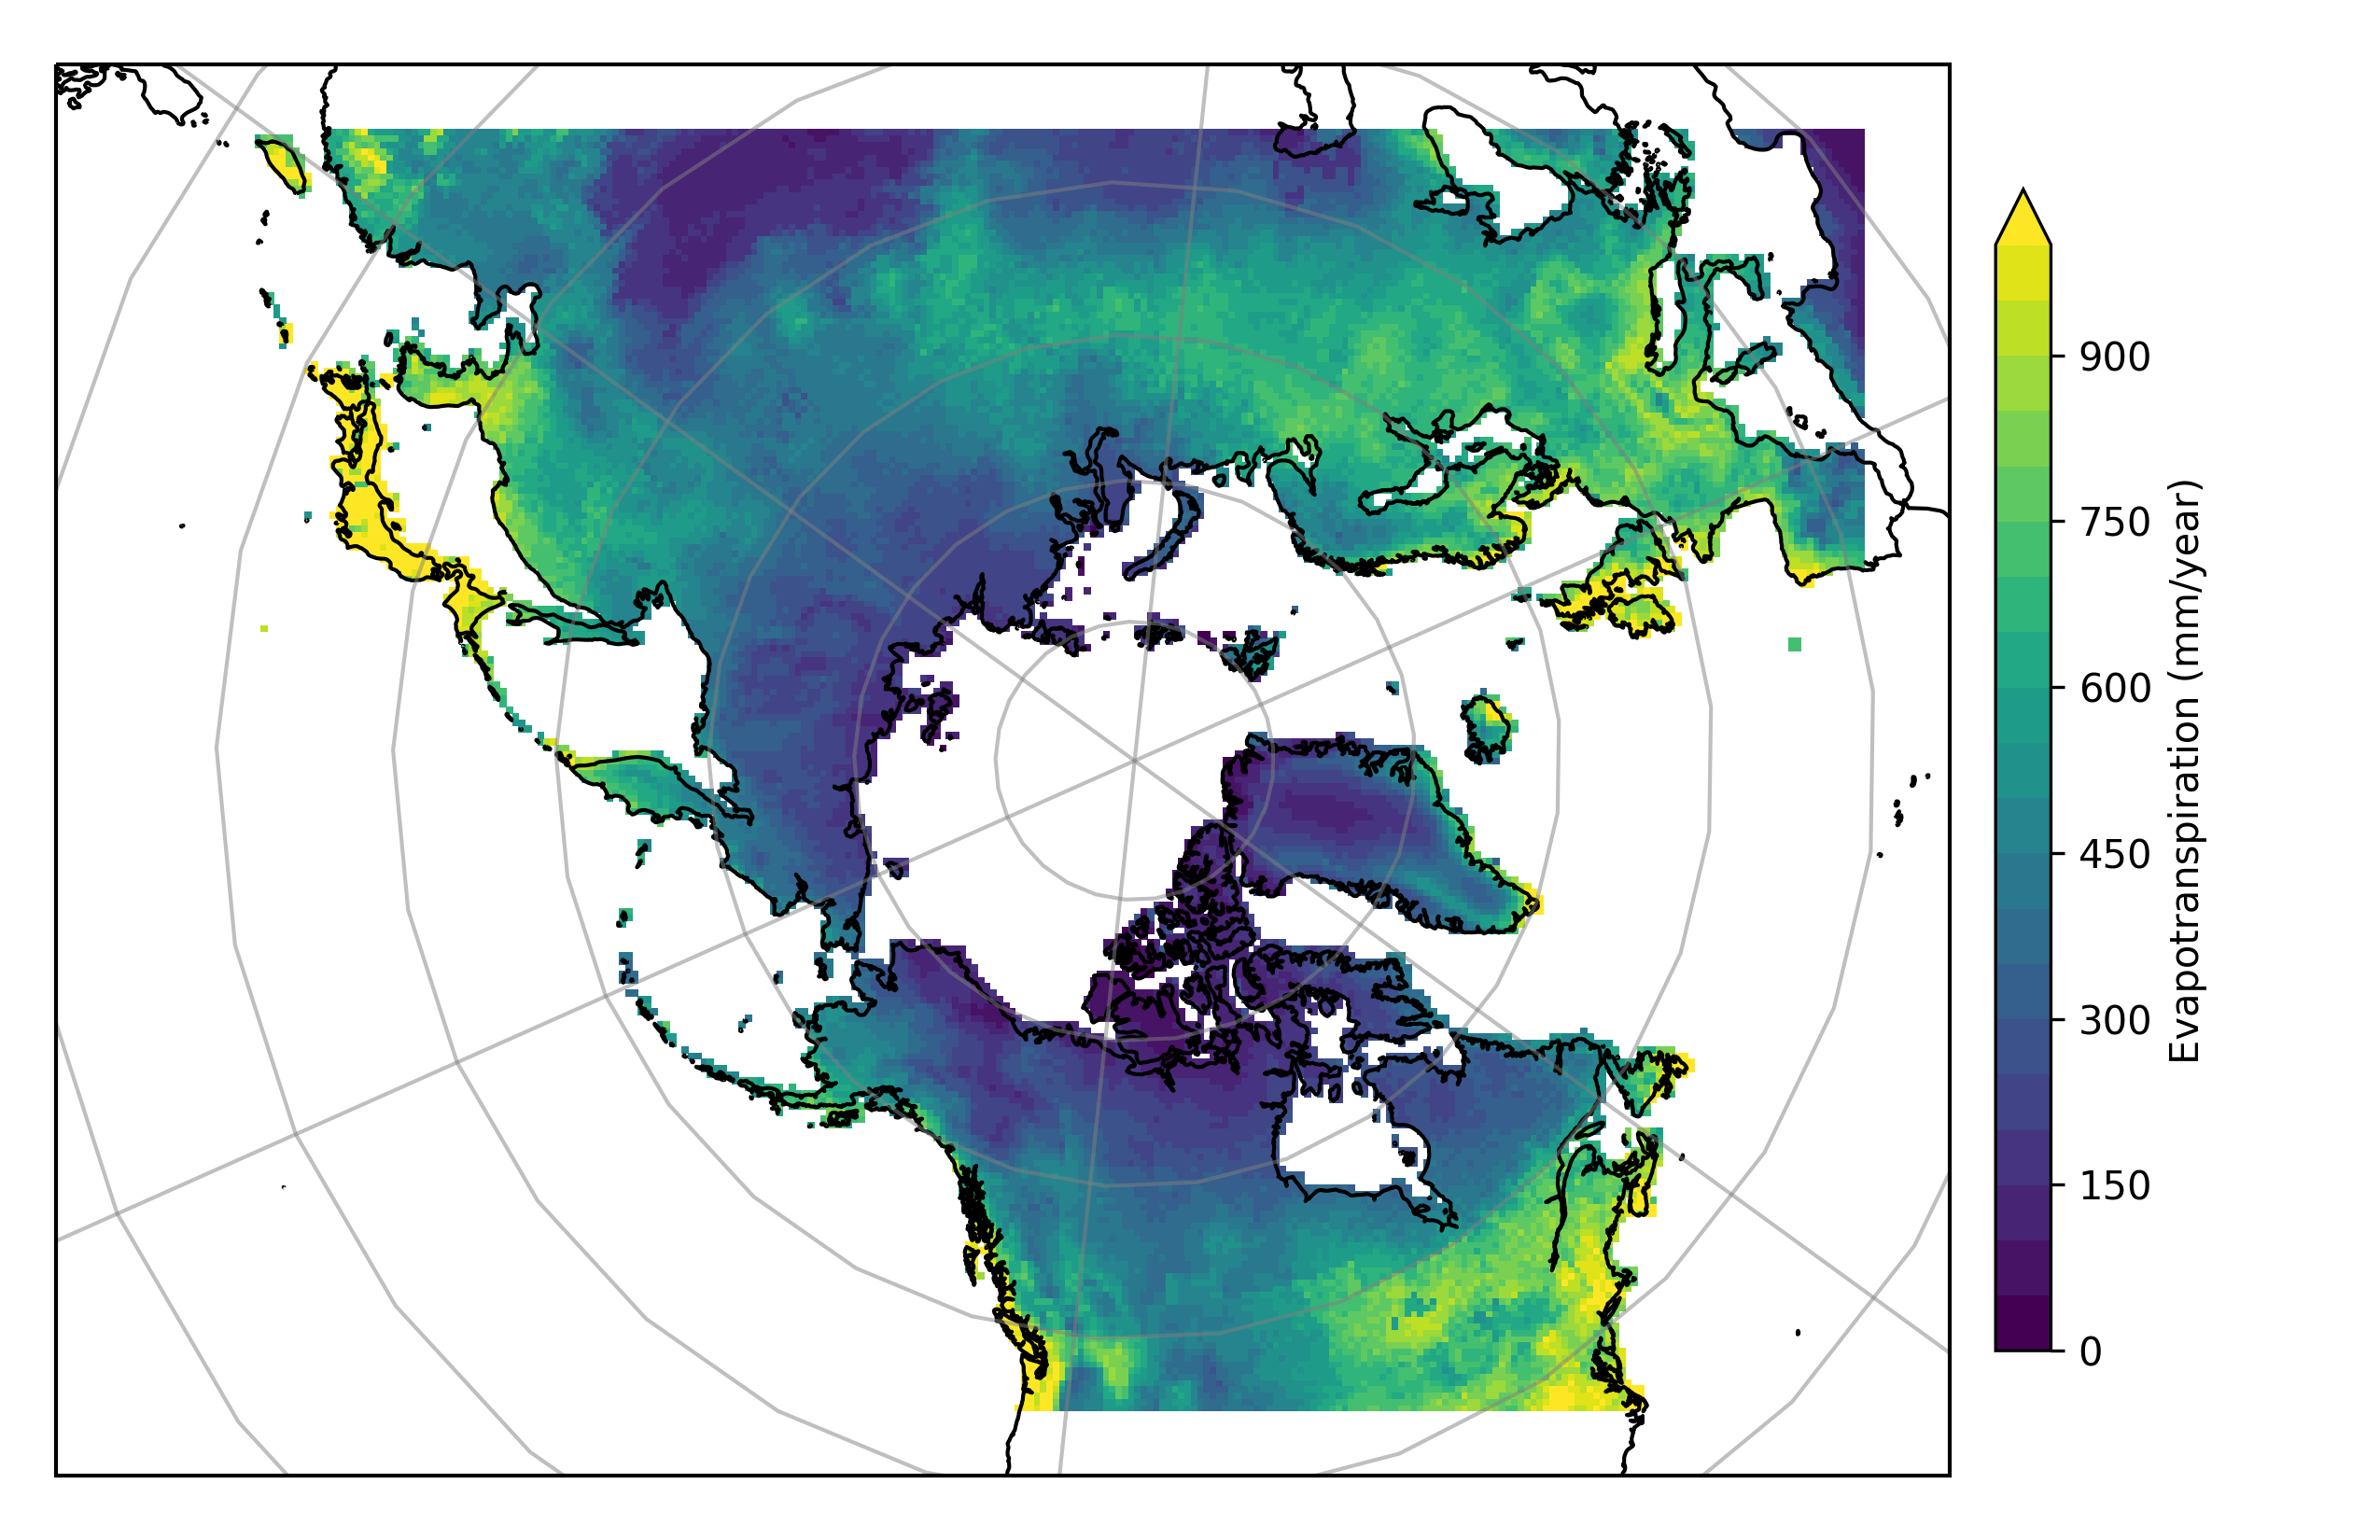
\includegraphics[width=6in]{RASM_domain_fig.png}
\caption{The 50-km near equal-area Regional Arctic System Model (RASM) domain. The model domain is comprised of 25,996 grid cells. }
\label{fig:vic_domain}
\end{figure}

\clearpage
\begin{figure}[t]
**- Use easier-to-read colors/patterns - e.g. solid lines for WB, dashed lines for EB;
- Use A & B (instead of EB & WB) to be consistent with text;
- The text doesn't mention the frozen soil option nor the number of nodes. Make the content of this figure consistent with the description in the text.**
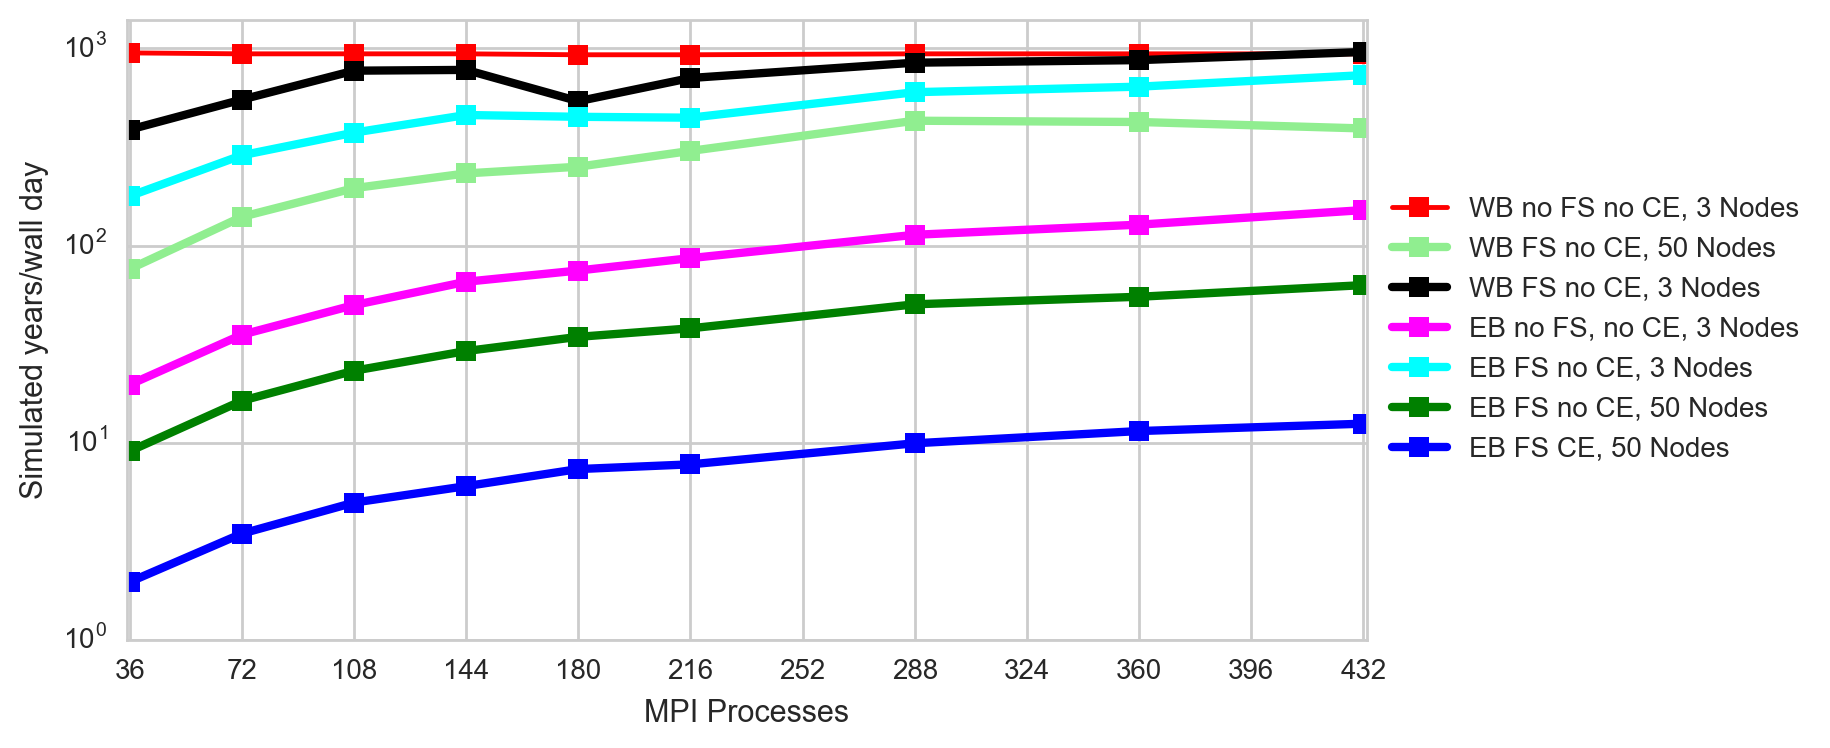
\includegraphics[width=6in]{VIC_scaling.png}
\caption{Model throughput for the seven model configurations run on the Thunder (SGI Ice X) and Gordon (Cray XC40) supercomputers.}
\label{fig:vic_scaling}
\end{figure}

\clearpage
\begin{figure*}[t]
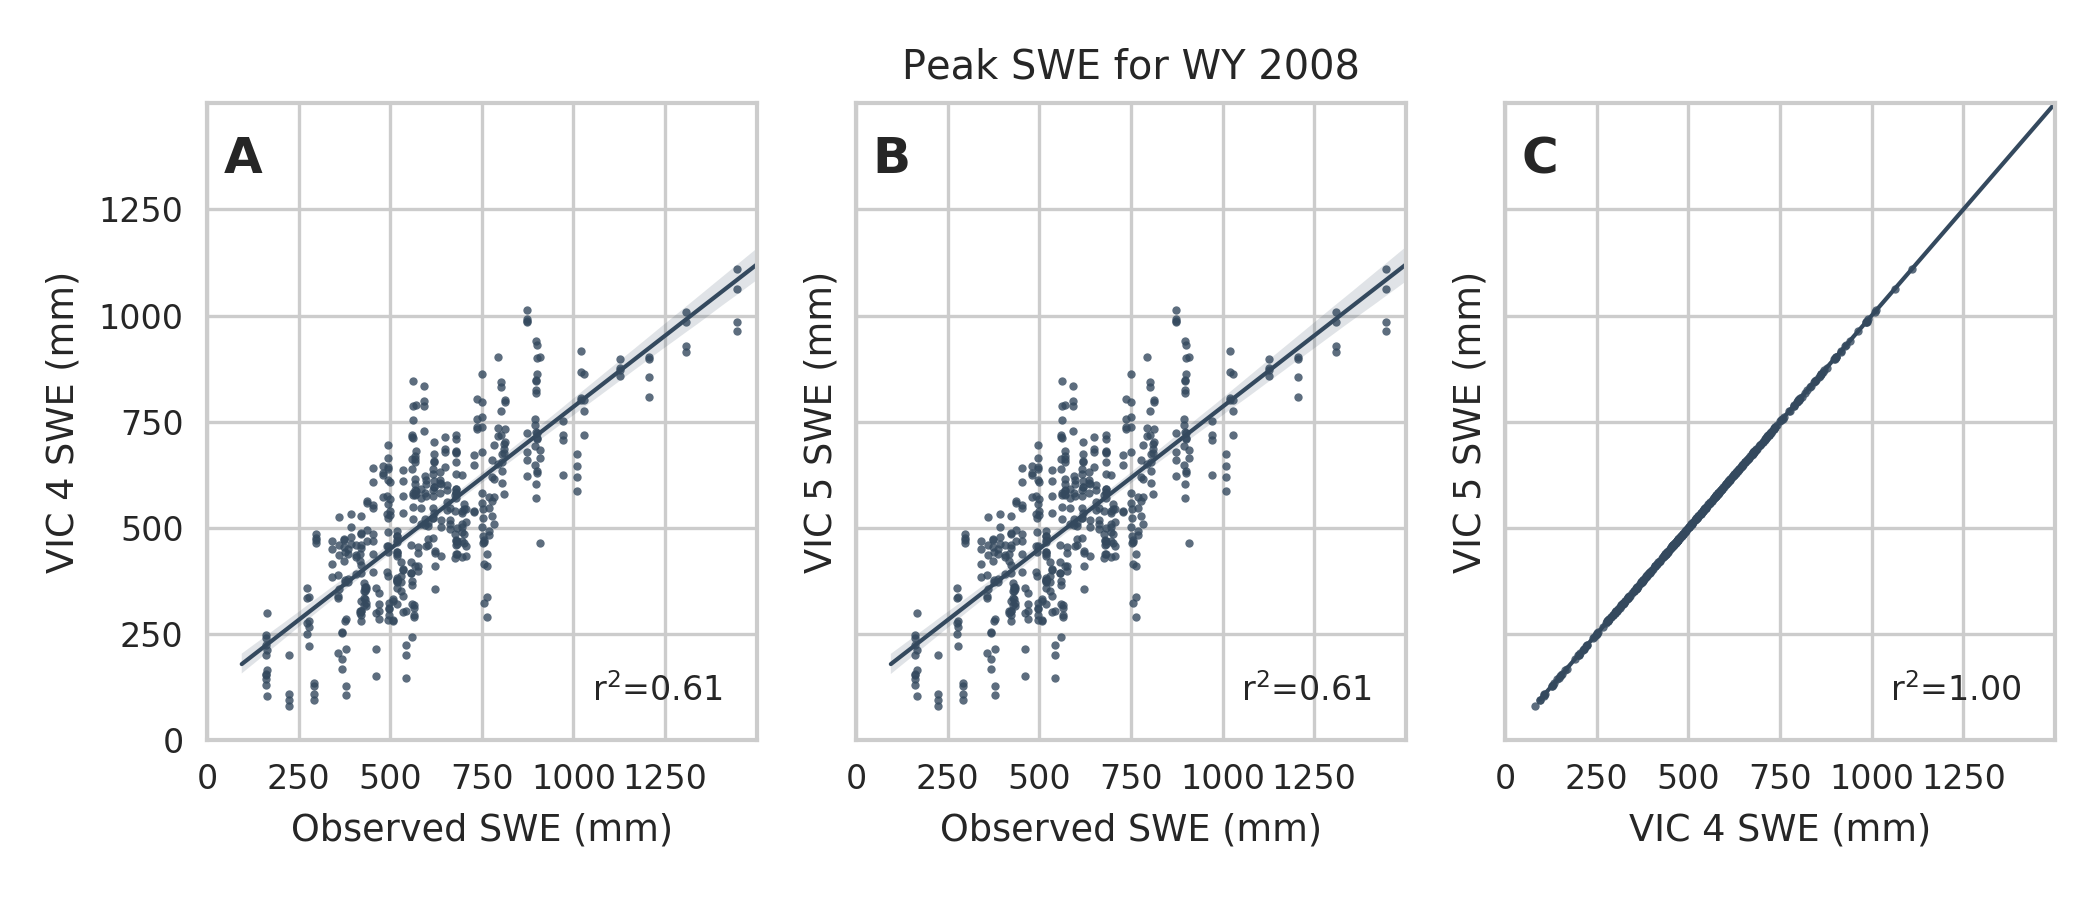
\includegraphics[width=6in]{VIC_science_tests_SWE.png}
\caption{Example summary figure from the VIC-5 SNOTEL science tests. A and B compare the results from VIC-4 and VIC-5 simulations with observations, respectively. C compares the the results from the two VIC versions.}
\label{fig:vic_4v5}
\end{figure*}

\clearpage
\begin{figure*}[t]
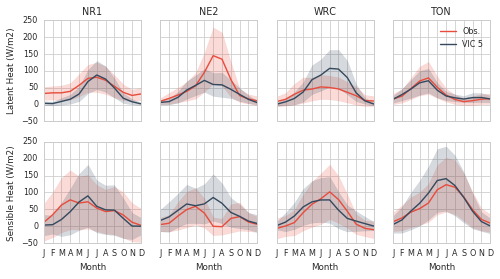
\includegraphics[width=12cm]{VIC_science_tests_fluxes.png}
\caption{Example summary output from the VIC-5 science testing package comparing the annual cycle of latent heat (top) and sensible heat (bottom) for four sample locations from VIC-5 (blue) to FluxNet observations (red).}
\label{fig:vic_fluxes}
\end{figure*}

%
%
%%% TABLES
%%%
%%% The different columns must be seperated with a & command and should
%%% end with \\ to identify the column brake.
%
%%% ONE-COLUMN TABLE
%
\clearpage
\begin{table}[]
  \caption{Examples of VIC applications}
  \label{table:vic_applications}
  \resizebox{\textwidth}{!}{%
  \begin{tabular}{ll}
    \hline
    \multicolumn{2}{l}{\textbf{Data set construction}}                                                                                                              \\ \hline
    \multicolumn{1}{l|}{US}                      & \citet{Maurer_2002}  \\ \hline
    \multicolumn{1}{l|}{Global}                  & \citet{Nijssen_2001a,Nijssen_2001c,Sheffield_2006}  \\ \hline
    \multicolumn{1}{l|}{Arctic}                  & \citet{Hamman_2017a} \\ \hline
    \multicolumn{2}{l}{\textbf{Historic trend analysis}}                                                                                                            \\ \hline
    \multicolumn{1}{l|}{Snow}                    & \citet{Hamlet_2005,Shi_2011}  \\ \hline
    \multicolumn{1}{l|}{Land use/cover change}   & \citet{Matheussen_2000}  \\ \hline
    \multicolumn{1}{l|}{Streamflow}              & \citet{Hamlet_2007a,Hamlet_2007b,Tan_2011}  \\ \hline
    \multicolumn{1}{l|}{Drought}                 & \citet{Gao_2011,Sheffield_2007,Sheffield_2008,Sheffield_2009,Wang_2011,Nijssen_2014}  \\ \hline
    \multicolumn{2}{l}{\textbf{Data evaluation}}                                                                                                                    \\ \hline
    \multicolumn{1}{l|}{Satellite precipitation} & \citet{Nijssen_2004,Pan_2010,Su_2008}  \\ \hline
    \multicolumn{1}{l|}{Reanalysis}              & \citet{Maurer_2001}  \\ \hline
    \multicolumn{2}{l}{\textbf{Data assimilation}}                                                                                                                  \\ \hline
    \multicolumn{1}{l|}{Snow}                    & \citet{Andreadis_2006}  \\ \hline
    \multicolumn{1}{l|}{Soil moisture}           & \citet{Pan_2006}  \\ \hline
    \multicolumn{2}{l}{\textbf{Forecasting and nowcasting}}                                                                                                         \\ \hline
    \multicolumn{1}{l|}{Droughts}                & \citet{Shukla_2011}  \\ \hline
    \multicolumn{1}{l|}{Streamflow}              & \citet{Hamlet_1999,Li_2009,Wood_2002}  \\ \hline
    \multicolumn{1}{l|}{Predictability}          & \citet{Gebregiorgis_2011,Maurer_2003}  \\ \hline
    \multicolumn{2}{l}{\textbf{Climate change impact analysis}}                                                                                                     \\ \hline
    \multicolumn{1}{l|}{Hydrology}               & \citet{Barnett_2005,Beyene_2010,Nijssen_2001b}  \\ \hline
    \multicolumn{1}{l|}{Water resources}         & \citet{Christensen_2007,Christensen_2004,Das_2011,Hamlet_1999}  \\ \hline
    \multicolumn{2}{l}{\textbf{Coupled land-atmosphere modeling}}                                                                                                     \\ \hline
    \multicolumn{1}{l|}{US}                      & \citet{Zhu_2009}                                           \\ \hline
    \multicolumn{1}{l|}{Arctic}                  & \citet{Hamman_2016a} \\ \hline
  \end{tabular}
  }
\end{table}

% Please add the following required packages to your document preamble:
% \usepackage{multirow}
\clearpage
\begin{table}[]
**Make this table the same format as Table 1**
**What is "Build" test? I guess it's to test if the code builds, but not mentioned in the text.**
**Need to fill in the question marks**
\centering
\caption{Summary of tests and datasets.}
\label{table:tests}
\resizebox{\textwidth}{!}{%
\begin{tabular}{|l|l|l|l|l|l|l|l|l|}
\hline
\textbf{Test type}                & \textbf{Driver}              & \textbf{Domain} & \textbf{Grid cells} & \textbf{Resolution} & \textbf{Timestep} & \textbf{Forcings}      & \textbf{Parameters} & \textbf{On Travis}  \\ \hline
\textbf{Build}                    & Classic, Image, CESM, Python & -               & -                   & -                   & -                 & -                      & -                   & yes                 \\ \hline
\textbf{Unit}                     & Python                       & -               & -                   & -                   & -                 & -                      & -                   & yes                 \\ \hline
\textbf{System}                   & Classic, Image, CESM         & Stehekin        & 16                  & 1/8-deg.            & 1-hour            & Maurer et al., 2002    & Maurer et al., 2002 & yes                 \\ \hline
\multirow{2}{*}{\textbf{Science}} & \multirow{2}{*}{Classic}     & SNOTEL          & 448 point locations & point               & 1-hour            & in-situ observations   & ?                   & \multirow{2}{*}{no} \\ \cline{3-8}
                                  &                              & FLUXNET         & 66 point locations  & point               & 1-hour            & in-situ observations   & ?                   &                     \\ \hline
\textbf{Examples}                 & Classic, Image               & Stehekin        & 16                  & 1/8-deg.            & 1-hour            & Maurer et al., 2002    & Maurer et al., 2002 & yes                 \\ \hline
\multirow{3}{*}{\textbf{Release}} & \multirow{3}{*}{Image}       & Global          & 61,345              & 1/2-deg.            & 6-hour            & CRU-NCEP               & Adam et al., 2006   & \multirow{3}{*}{no} \\ \cline{3-8}
                                  &                              & N. America      & 333,579             & 1/16-deg.           & 3-hour            & Livneh et al., 2015    & Livneh et al., 2015 &                     \\ \cline{3-8}
                                  &                              & RASM            & 25,996              & 50-km               & 3-hour            & Sheffield et al., 2006 & Hamman et al., 2016 &                     \\ \hline
\textbf{Performance}              & Image                        & RASM            & 25,996              & 50-km               & 3-hour            & Sheffield et al., 2006 & Hamman et al., 2016 & no                  \\ \hline
\end{tabular}
}
\end{table}

\clearpage
\begin{table}[]
\centering
\caption{Hardware used in VIC Image driver parallel scaling performance tests.}
\label{table:hardware}
**Make this table the same format as Table 1**
\resizebox{\textwidth}{!}{%
\begin{tabular}{|l|l|l|}
\hline
\textbf{}                                & \textbf{Thunder}                            & \textbf{Cheyenne}                           \\ \hline
\textbf{Operated By}                     & Air Force Research Laboratory (AFRL)        & National Center for Atmospheric Research (NCAR) \\ \hline
\textbf{System}                          & SGI ICE X                                   & SGI ICE XA                                  \\ \hline
\textbf{Peak PFlops}                     & 5.62                                        & 5.34                                        \\ \hline
\textbf{Parallel disk storage (Pbytes)}  & 12.2                                        & 52.7                                        \\ \hline
\textbf{Total Nodes}                     & 3,216                                       & 4,032                                       \\ \hline
\textbf{Cores per Node}                      & 36                                          & 36                                          \\ \hline
\textbf{Core Type}                       & Intel Xeon E5-2699v3                        & Intel Xeon E5-2697V4                        \\ \hline
\textbf{Core Speed (GHz)}                & 2.3                                         & 2.3                                         \\ \hline
\textbf{Memory/Node (Gbytes)}            & 128                                         & 64 or 128                                   \\ \hline
\textbf{Memory Model}                    & Shared on node. Distributed across cluster. & Shared on node. Distributed across cluster. \\ \hline
\textbf{Interconnect Type}               & FDR 14x InfiniBand / Enhanced LX Hypercube  & Mellanox EDR InfiniBand                     \\ \hline
\end{tabular}
}
\end{table}
%
%%% NUMBERING OF FIGURES AND TABLES
%%%
%%% If figures and tables must be numbered 1a, 1b, etc. the following command
%%% should be inserted before the begin{} command.
%
%\addtocounter{figure}{-1}\renewcommand{\thefigure}{\arabic{figure}a}
%
%
%%% MATHEMATICAL EXPRESSIONS
%
%%% All papers typeset by Copernicus Publications follow the math typesetting regulations
%%% given by the IUPAC Green Book (IUPAC: Quantities, Units and Symbols in Physical Chemistry,
%%% 2nd Edn., Blackwell Science, available at: http://old.iupac.org/publications/books/gbook/green_book_2ed.pdf, 1993).
%%%
%%% Physical quantities/variables are typeset in italic font (t for time, T for Temperature)
%%% Indices which are not defined are typeset in italic font (x, y, z, a, b, c)
%%% Items/objects which are defined are typeset in roman font (Car A, Car B)
%%% Descriptions/specifications which are defined by itself are typeset in roman font (abs, rel, ref, tot, net, ice)
%%% Abbreviations from 2 letters are typeset in roman font (RH, LAI)
%%% Vectors are identified in bold italic font using \vec{x}
%%% Matrices are identified in bold roman font
%%% Multiplication signs are typeset using the LaTeX commands \times (for vector products, grids, and exponential notations) or \cdot
%%% The character * should not be applied as mutliplication sign
%
%
%%% EQUATIONS
%
%%% Single-row equation
%
%\begin{equation}
%
%\end{equation}
%
%%% Multiline equation
%
%\begin{align}
%& 3 + 5 = 8\\
%& 3 + 5 = 8\\
%& 3 + 5 = 8
%\end{align}
%
%
%%% MATRICES
%
%\begin{matrix}
%x & y & z\\
%x & y & z\\
%x & y & z\\
%\end{matrix}
%
%
%%% ALGORITHM
%
%\begin{algorithm}
%\caption{�}
%\label{a1}
%\begin{algorithmic}
%�
%\end{algorithmic}
%\end{algorithm}
%
%
%%% CHEMICAL FORMULAS AND REACTIONS
%
%%% For formulas embedded in the text, please use \chem{}
%
%%% The reaction environment creates labels including the letter R, i.e. (R1), (R2), etc.
%
%\begin{reaction}
%%% \rightarrow should be used for normal (one-way) chemical reactions
%%% \rightleftharpoons should be used for equilibria
%%% \leftrightarrow should be used for resonance structures
%\end{reaction}
%
%
%%% PHYSICAL UNITS
%%%
%%% Please use \unit{} and apply the exponential notation


\end{document}
